\documentclass{article}

\usepackage[polish]{babel}
\usepackage[utf8]{inputenc}
\usepackage{polski}

\usepackage{amsmath}
\DeclareMathOperator{\sgn}{sgn}

\usepackage{pgfplots}
\pgfplotsset{compat=1.17}

\graphicspath{ {./images/} }

\title{Klasyfikacja COVID-19 na zdjęciach rentgenowskich}
\author{Vladyslav Diachuk s18901}

\bibliographystyle{plain}

\makeindex
\begin{document}
\maketitle

%===================================================================================
\section{Wstęp}

%-----------------------------------------------------------------------------------
\subsection{Abstrakt}


%-----------------------------------------------------------------------------------
\subsection{Słowa kluczowe}


%-----------------------------------------------------------------------------------
\subsection{Teza główna}

%-----------------------------------------------------------------------------------
\subsection{Motywacja}


%===================================================================================
\section{Choroby płuc, rozpoznawanie, skutki}

%===================================================================================
\section{Uczenie maszynowe}
Uczeniem maszynowym nazywa się dziedzina nauki (i sztukę) programowania komputerów w sposób umożliwiający im uczenie się z danych \cite{geron} 
Ta praca jest zrobiona z użyciem uczenia maszynowego a zwłaszcza sieci neuronowych.


%===================================================================================
\section{Neuron}
Zanim opiszę sieci neuronowe, chcę przedstawić co to jest neuron (komórka).

\subsection{Neuron biologiczny}
Jak wiadomo mózg ludzki i większości innych organizmów składa się z malutkich komórek nerwowych, nazywanych neuron, zdolnych do przetwarzania i przewodzenia informacji w postaci sygnału elektrycznego. Neurony są podstawowym elementem układu nerwowego zwierząt. Najwięcej neuronów znajduje się w ośrodkowym układzie nerwowym, w skład którego wchodzi mózgowie oraz rdzeń kręgowy. \cite{neuroscience}
Głównymi elementami neuronu są ciało komórki zawierające jądro i większość organelli komórkowych, wiele rozgałęziających się wypustek zwanych dendrytami oraz jedna bardzo długa wypustka -- akson. \cite{geron}

\begin{figure}
	\centering
	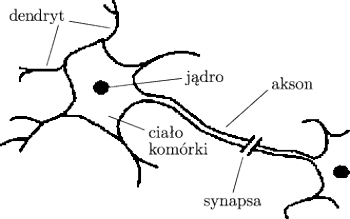
\includegraphics[width=\textwidth,height=6cm,keepaspectratio=true]{neuron_bio}
	\caption{
		Obraz komórki biologicznej \cite{neuron_bio}
	}
\end{figure}

Neurony biologiczne generują krótkie impulsy elektryczne zwane sygnałami, które są przenoszone wzdłuż aksonów i powodują uwalnianie w synapsach sygnałów chemicznych zwanych neuroprzekaźnikami. Kiedy komórka nerwowa otrzymuje dostateczną liczbę neuroprzekaźników od innych neuronów w ciągu kilku milisekund, to sama zaczyna wysyłać własne sygnały elektryczne (w rzeczywistości jest to uzależnione od neuroprzekaźników, gdyż niektóre z nich hamują aktywność komórki nerwowej). \cite{geron}
Zatem mechanizm działania poszczególnych neuronów jest dość prosty, tworzą one jednak rozległą sieć składającą się z miliardów komórek nerwowych, gdzie zazwyczaj jeden neuron łączy się z tysiącami innych. Dzięki tak olbrzymiej sieci zawierającej proste komórki nerwowe mogą być wykonywane skomplikowane obliczenia.

\subsection{Sztuczny neuron}
W 1943 przez Warren S. McCulloch i Walter Pitts było zaproponowano bardzo prostą reprezentację neuronu sztucznego. On ma co najmniej jedno binarne wejście i dokładnie jedno binarne wyjście. Wyjście zostanie aktywne tylko wtedy kiedy będzie aktywna określona liczba wejść. \cite{mcculloch1943logical} Tak prosty model daje nam bardzo duże możliwości. Twórcy udowodnili że za pomocą takich neuronów jesteśmy w stanie zaprotestować sieć która rozwiąże dowolne zadanie logiczne.

\clearpage
	
\begin{figure}
	\centering
	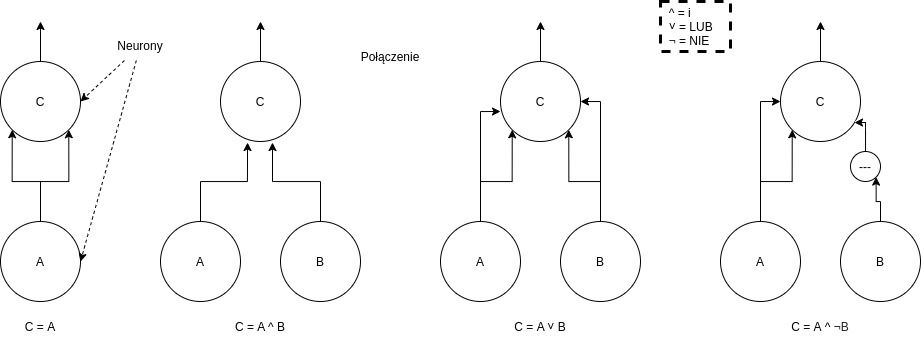
\includegraphics[width=\textwidth,keepaspectratio=true]{SSN_simple_neurons}
	\caption{
		Przykład sztucznych sieci neuronowych przeprowadzających proste operacje logiczne. Neuron aktywuje się przy co najmniej dwóch aktywnych wejściach \cite{geron}
	}
\end{figure}

Frank Rossenblatt trochę zmodyfikował ten neuron.\newline
Kluczowe zmiany:
\begin{itemize}
	\item Wartościami wejść/wyjść są liczby
	\item Każde połączenie ma przyporządkowaną wagę.
	\item Używanie funkcji skokowej na końcu
	\item Dodatkowe obciążeniowe wejście(zawsze wysyła wartość 1) z własną wagą, tak zwany bias
\end{itemize}
Jednostka wylicza ważoną sumę sygnałów wejściowych, a następnie zostaję użyta funkcja aktywacji. Najczęściej zostaje użyta funkcja skokowa Heaviside`a lub signum.Przy użyciu skokowej funkcji aktywacji taki neuron można nazywać progową jednostką logiczną lub liniową jednostką progową (ang. \textit{Linear Treshod Unit} -- LTU). Dziawanie tej jednoki można matematycznie opisać w następujący sposób.\newline\newline
$ y = \mathcal{H}(W^{T}X + b) $\newline \newline
Gdzie: \newline
X -- wektor wejść. \newline
W -- wektor wag. \newline
b -- bias. \newline
y -- wyjście neuronu. \newline
$ \mathcal{H}(...) $ -- funkcja skokowa Heaviside`a\newline

\begin{figure}[!ht]
	\centering
	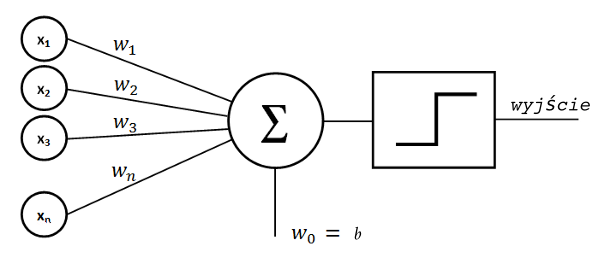
\includegraphics[width=0.8\textwidth,keepaspectratio=true]{neuron_rosenblatta}
	\caption{
		Sztuczny neuron Franka Rosenblatta
	}
\end{figure}


%===================================================================================
\section{Funkcji aktywacji użyte w pracy}

\begin{center}
	Signum\newline
	\begin{tikzpicture}
		\begin{axis}[
			axis lines=middle,
			xlabel=$x$,
			ylabel={$y$},
			xmin=-3, xmax=3,
			ymin=-1.5, ymax=1.5,
			xtick={-1, 0, 1},
			ytick={0, 1},
			extra y ticks={-1},
			extra y tick style={
				tick label style={anchor=west, xshift=3pt},
			},
			function line/.style={
				red,
				thick,
				samples=2,
			},
			single dot/.style={
				red,
				mark=*,
			},
			empty point/.style={
				only marks,
				mark=*,
				mark options={fill=white, draw=black},
			},
			]
			\addplot[function line, domain=\pgfkeysvalueof{/pgfplots/xmin}:0] {-1};
			\addplot[function line, domain=0:\pgfkeysvalueof{/pgfplots/xmax}] {1};
			\addplot[single dot] coordinates {(0, 0)};
			\addplot[empty point] coordinates {(0, -1) (0, 1)};
		\end{axis}
	\end{tikzpicture}
\end{center}

\begin{center}
	Funkcja skokowa Heaviside`a\newline
	\begin{tikzpicture}
		\begin{axis}[
			axis lines=middle,
			xlabel=$x$,
			ylabel={$y$},
			xmin=-3,
			xmax=3,
			xtick={-1, 0, 1},
			axis x line=bottom,
			ytick={0,1},
			ymax=1.5,
			axis y line=middle,
			function line/.style={
				red,
				thick,
				samples=2,
			},
			single dot/.style={
				red,
				mark=*,
			},
			empty point/.style={
				only marks,
				mark=*,
				mark options={fill=white, draw=black},
			},
			]
			\addplot[function line, domain=\pgfkeysvalueof{/pgfplots/xmin}:0] {0};
			\addplot[function line, domain=0:\pgfkeysvalueof{/pgfplots/xmax}] {1};
			\addplot[single dot] coordinates {(0, 0)};
			\addplot[empty point] coordinates {(0, 1)};
		\end{axis}
	\end{tikzpicture}
\end{center}

\begin{center}
	\begin{tikzpicture}
		\begin{axis}[
			axis lines=middle,
			xlabel=$x$,
			ylabel=$y$,
			xmin=-3, xmax=3,
			ymin=-3, ymax=3,
			xtick={1, 0},
			ytick={0, 1},
			function line/.style={
				red,
				thick,
				samples=2,
			},
			single dot/.style={
				red,
				mark=*,
			},
			empty point/.style={
				only marks,
				mark=*,
				mark options={fill=white, draw=black},
			},
			]
			\addplot[function line, domain=\pgfkeysvalueof{/pgfplots/xmin}:0] {0};
			\addplot[function line, domain=0:\pgfkeysvalueof{/pgfplots/xmax}] {x};
		\end{axis}
	\end{tikzpicture}	
\end{center}

\begin{center}
	\begin{tikzpicture}[declare function={sigma(\x)=1/(1+exp(-\x));
			sigmap(\x)=sigma(\x)*(1-sigma(\x));}]
		\begin{axis}%
			[     
			xmin=-6,
			xmax=6,
			axis x line=bottom,
			ytick={0,.5,1},
			ymax=1,
			axis y line=middle,
			samples=100,
			domain=-6:6,
			legend style={at={(1,0.9)}}     
			]
			\addplot[red,mark=none]   (x,{sigma(x)});
			\addplot[blue,dotted,mark=none]   (x,{sigmap(x)});
			\legend{$\sigma(x)$,$\sigma'(x)$}
		\end{axis}
	\end{tikzpicture}
\end{center}


%===================================================================================
\section{Sieci neuronowe w klasyfikacji danych wizualnych}

%-----------------------------------------------------------------------------------
\subsection{Model neuronu jako klasyfikator}

%-----------------------------------------------------------------------------------
\subsection{Konwolucyjne sieci neuronowe}

%-----------------------------------------------------------------------------------
\subsection{Uczenie sztucznych sieci neuronowych}



%===================================================================================
\section{Architektura konwolucyjna w detekcji chorób płuc}



\bibliography{bibliografia}

	
\end{document}